\section{Results}
\label{sec:results}

In the following sections, we explore the response of the log-loss and Brier score metrics to the presence of classifier error properties and as a function of the weighting scheme on the class(es) affected by each systematic.

\subsection{Mock classifier systematics}
\label{sec:mockresults}

\begin{figure*}
	\begin{center}
		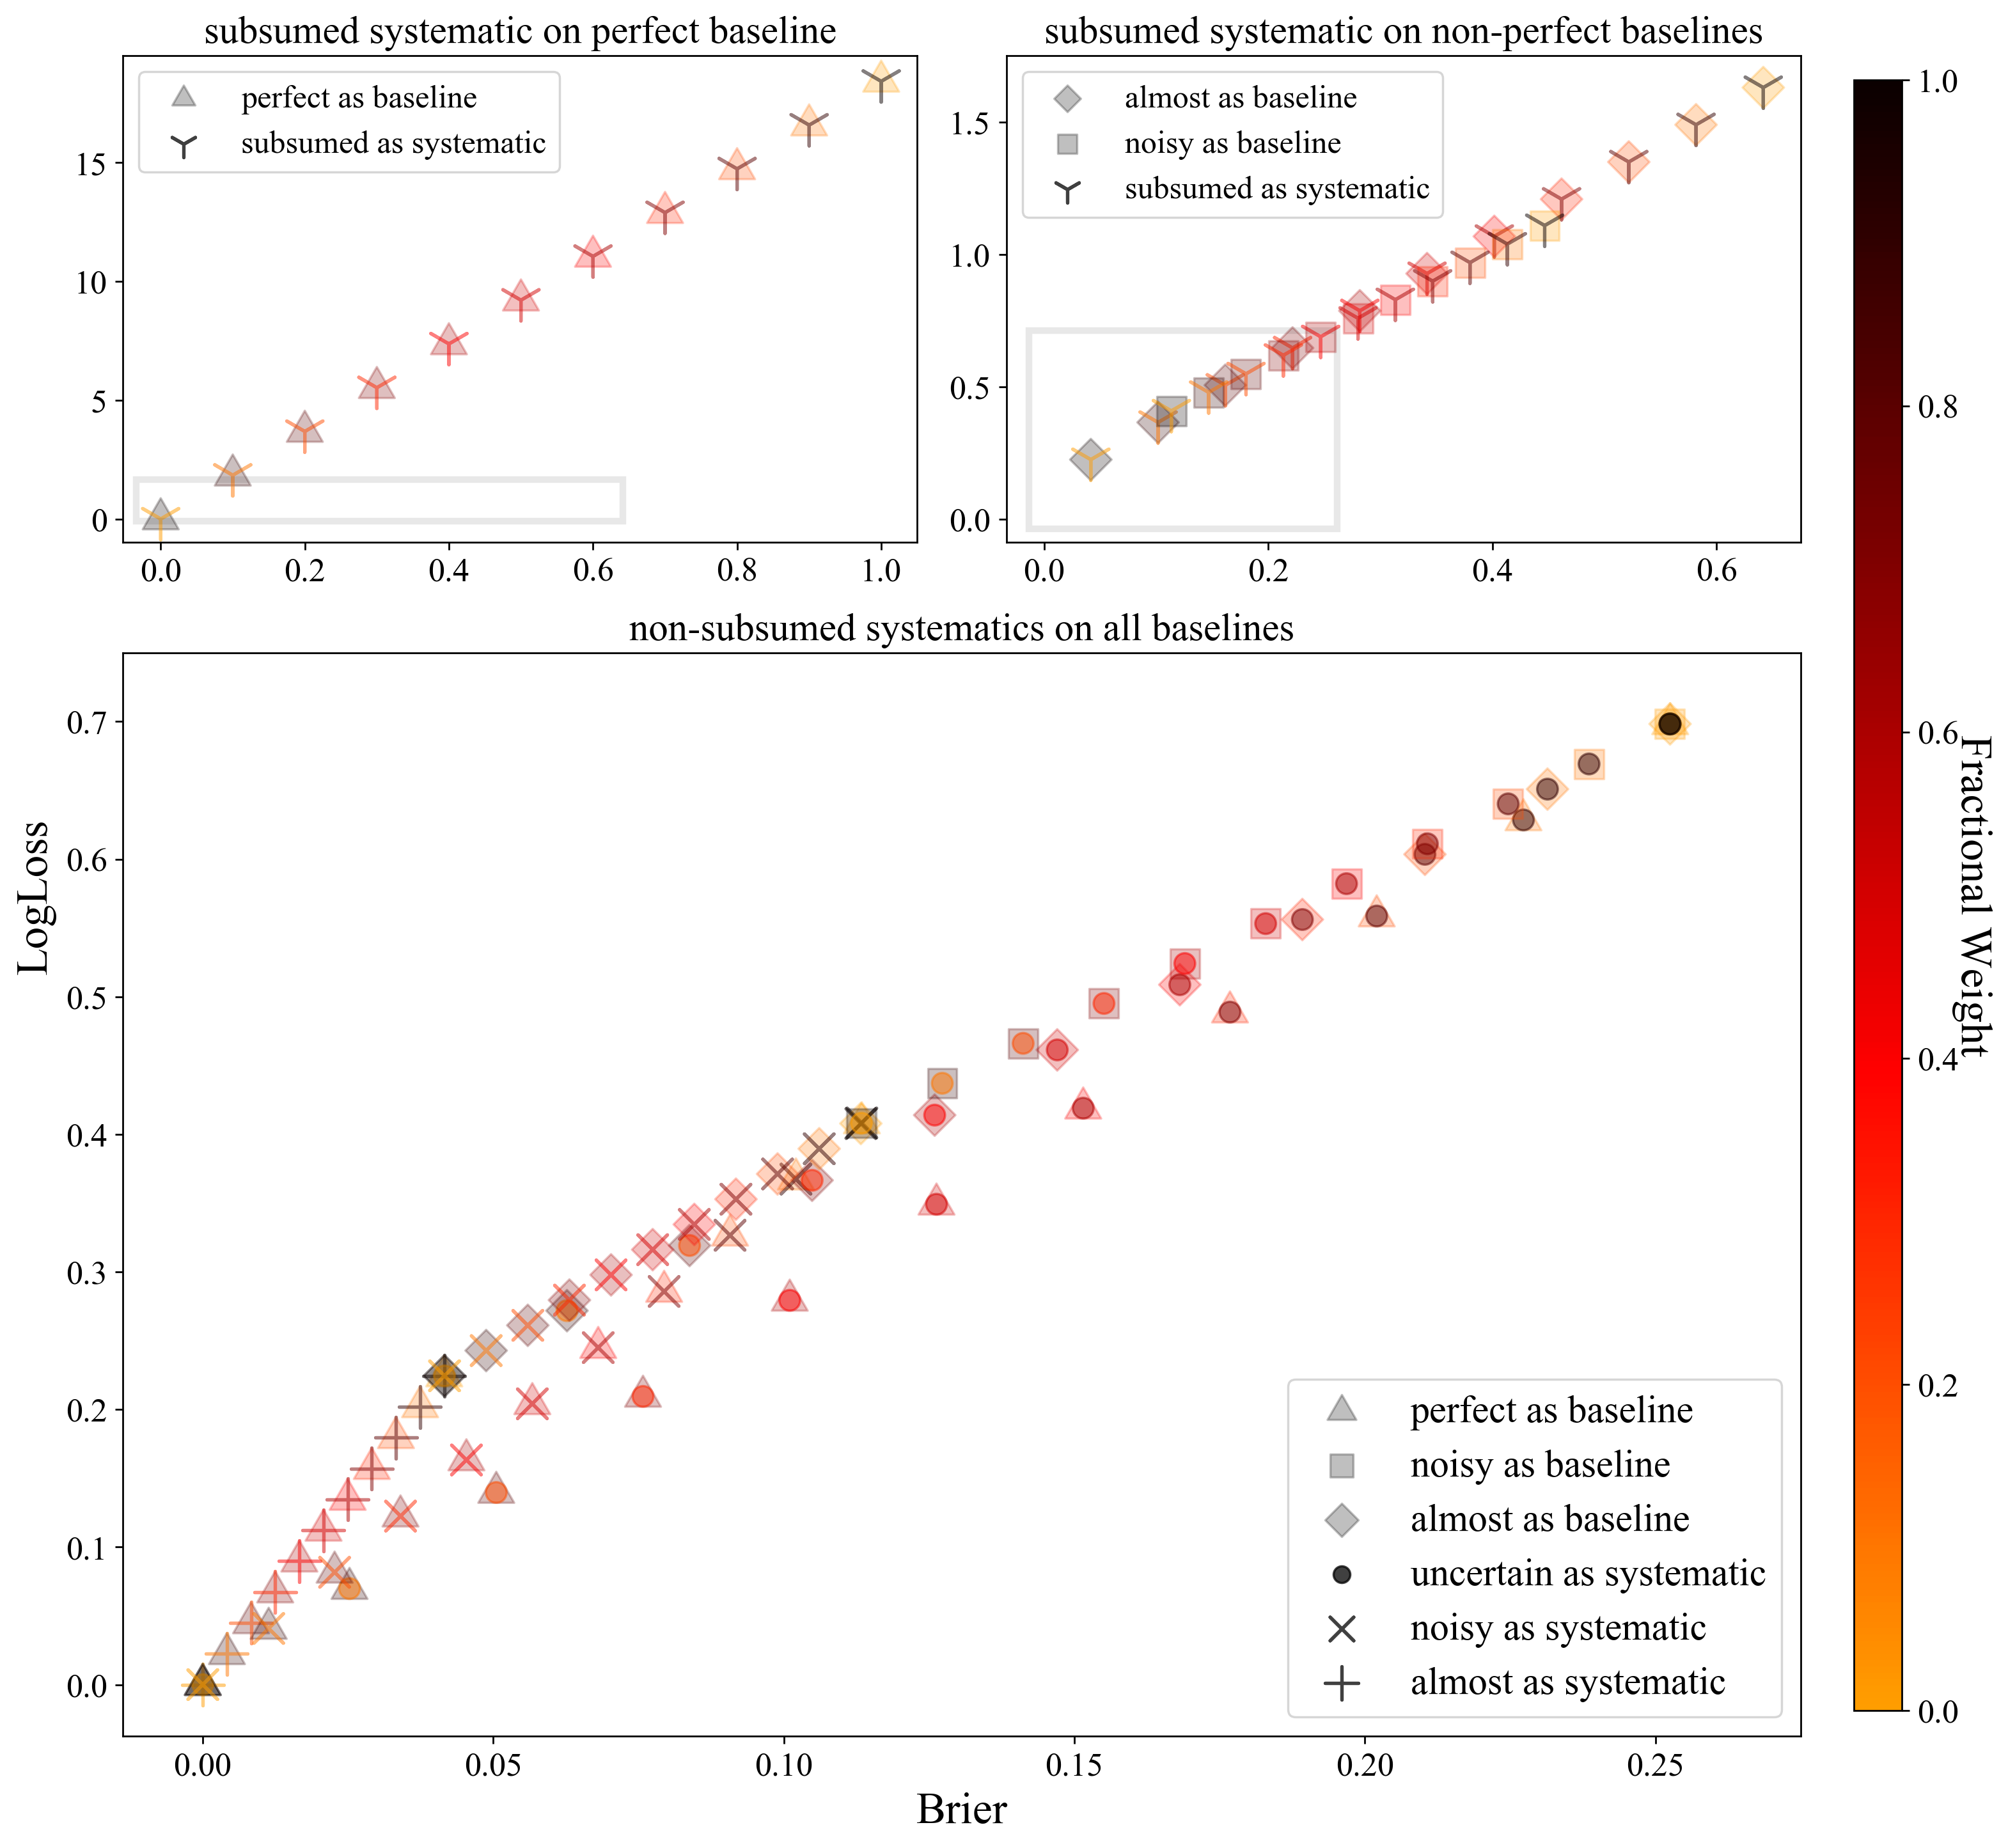
\includegraphics[width=0.95\textwidth]{./fig/multipanel_res.png}
		\caption{Weighted log-loss and Brier scores for classifiers with combinations of systematics.
		Each point represents a classifier with baseline behavior (regular polygon marker) for all but one class with a particular systematic (asterisk markers).
		The color of the systematic effect and baseline behavior markers indicates the weight on the class affected by the systematic and the integrated weight evenly distributed over other classes with baseline behavior, respectively.
		The $x$-axis is the Brier score and the $y$-axis is the log-loss.
		\aim{TODO: Update caption for new plot.}
		}
	\end{center}
	\label{fig:all_combined}
\end{figure*}

We simulate mock classifications from linear combinations of the conditional probability matrices using logarithmically distributed class populations to make a catalog of $10^{6}$ posterior probability vectors for every conditional probability matrix, as described in of Section~\ref{sec:mockdata}.
In Figure~\ref{fig:all_combined}, we demonstrate the behavior of the metrics with classification posteriors derived from conditional probability matrices composed of pairs of baseline classifier error properties.
The baselines considered are the uncertain, perfect, almost perfect, and noisy conditional probability matrices described in Section~\ref{sec:mockdata}.
The systematics introduced to each baselines are those that we intuitively expect to worsen performance, as considering all combinations would be redundant;
the uncertain, almost perfect, noisy, and subsuming classifiers are anticipated to worsen an otherwise perfect classifier;
the uncertain, noisy, and subsuming classifiers are anticipated to worsen an otherwise almost perfect classifier;
the uncertain and subsuming classifiers are anticipated to worsen an otherwise noisy classifier;
and the subsuming classifier is anticipated to worsen an otherwise uncertain classifier.
We also vary the weights placed on the class affected by the worsening systematic and the integrated weight of all other classes with baseline behavior, with values ranging from 0 (all weight on the baseline) to 1 (all weight on the systematic).
The variation in weights establishes linear relationships between the log-loss and Brier score metrics for each pair of baseline and systematic.

We note that for all weight on the perfect classifier, the values of both metrics vanish to zero.
It is immediately evident that the log-loss has more dynamic range than the Brier score overall, and that both metrics are acutely sensitive to the subsuming systematic on a baseline of a perfect classifier.
In fact, the log-loss value for a classifier that subsumes a class into one that is classified perfectly should actually be infinite and only takes a finite value because of the limits of floating point precision and our own restriction that no probabilities be below $10^{-8}$ chosen to ensure numerical stability.
Because the combination of a subsuming classifier with a perfect baseline is so different from all other combinations, we further separate the subsuming systematic with all other baselines (lower left panel) from all other systematics (lower right panel) in Figure~\ref{fig:all_combined}.

The range of the log-loss is greater than that of the Brier score in the two panels of Figure~\ref{fig:all_combined}, showing that the dynamic range of the log-loss remains higher even outside the regime where it tends toward infinity.
The extent of the values of both metrics is higher in the left panel with the subsuming systematic on various baselines than in the right panel with all other systematics.
This shows that both metrics are still more sensitive to the subsuming systematic than any other systematic, confirming that both can appropriately penalize the cruise control effect.
When all weight is on the class affected by a systematic, there is a characteristic limit for each metric's values, shown in Table~\ref{tab:extents}.
Because a subsumed class takes the conditional probability vector of the subsuming class, the metric values depend on what systematics may be affecting the subsuming class as well.
Based on Table~\ref{tab:extents}, both metrics would agree on the ranking of these classifiers, which we shall see is not a guarantee.
Furthermore, this invariant ranking is consistent with our intuition about the severity of anticipated faults of classifiers.

\begin{table}[]
\begin{tabular}{lll}
Mock classifier & Brier score & Log-loss\\
\hline
Perfect & 0.0 & 0.0\\
Almost perfect & 0.042 & 0.225\\
Noisy & 0.113 & 0.408\\
Uncertain & 0.253 & 0.699\\
Subsumed from Uncertain & 0.252 & 0.696\\
Subsumed from Noisy & 0.447 & 1.109\\
Subsumed from Almost & 0.641 & 1.629\\
Subsumed from Perfect & 1.0 & 18.421\footnote{The entry for the log-loss of a classifier that subsumes a class into one that is otherwise perfectly classified should be infinite but is bounded by the numerical precision of our calculations.}
\end{tabular}
\caption{The value of each metric when the weight is entirely on the class affected by each systematic.
Note that the differences in metric values for the uncertain classifier and the uncertain classifier affected by the subsuming systematic are not statistically significant.}
\label{tab:extents}
\end{table}

The slopes in Figure~\ref{fig:subsume}, however, represent the relative sensitivity ratio of the log-loss to the Brier score, and they differ for each baseline-systematic pair.
These values are given in Table~\ref{tab:slopes}, aside from the subsuming systematic on a baseline of an uncertain classifier, as it is not statistically significant.
The log-loss always has higher sensitivity than the Brier score, particularly to the difference between the perfect classifier and any lesser classifier.
A possible implication of this behavior is that the log-loss may have an enhanced ability to distinguish between multiple high-performing classifiers that might not have meaningfully different metric values under the Brier score.
In a sense, it means that the log-loss is more susceptible to the tunnel vision classifier, with a significant response to any move toward perfection.
% However, the slope is higher for the almost perfect systematic than the noisy systematic, and higher for the noisy systematic than the uncertain systematic; this means that a tunnel vision classifier is deprived of the metric's favor more if it neglects other classes than if it already does fairly well for them, a case in which we would not call it much of a systematic.

\begin{table}[]
\begin{tabular}{l|llll}
	& Systematics & & &\\
Baselines & Subsumed & Uncertain & Noisy & Almost\\
\hline
Perfect & 18.421 & 2.763 & 3.601 & 5.387\\
Almost perfect & 2.343 & 2.246 & 2.556 & \\
Noisy & 2.102 & 2.085 & & \\
% Uncertain & 2.013\footnote{As is indicated in the caption to Table~\ref{tab:extents}, the slope of the subsuming systematic on a baseline of uncertain classification is not statistically significant.} & & &
\end{tabular}
\caption{The slopes for each baseline-plus-systematic pair in the space of log-loss  versus Brier score.
A higher slope corresponds to increased sensitivity of the log-loss.}
\label{tab:slopes}
\end{table}

\aim{Still reworking past here.}
Consider a weighting of $\sim0.8$ for a class affected by tunnel vision, leaving $\sim0.2$ to be shared evenly among all other classes uniformly affected by the other systematics.
Qualitatively, we would say that a classifier that is almost perfect for other classes is superior to one that is noisy, and a classifier that is noisy for other classes is still superior to one that is uniform; furthermore, the subsuming classifier is even more harshly penalized in this situation than the uncertain classifier, meaning both metrics are  consistent with our basic tests of intuition in this case.
However, this observation also indicates that the tunnel vision systematic is difficult to penalize, and that if the affected class is given a large weight, it can easily dominate the metric.
If all classes are of scientific importance, heavily unequal weighting can incentivize tunnel vision classification.

% We introduced weighting of per-class metrics to discourage `tunnel vision' and `cruise control' classifiers that can ignore classes other than the most common and nonetheless perform well by a metric.
% Figure~\ref{fig:popweight} shows the impact of weighting the per-class metrics by the number of objects in the class as each is affected by one of the systematics and the other classes are held at the more realistic almost perfect performance.
% The points show different classification schemes, and all points are coloured by the change in the weighting, dependent on the size of the population class being classified.
% Conversely, the cruise control classifier and, to a lesser degree the noisy classifier, always has high log-loss and Brier score values regardless of the weight on the affected class.

% \begin{figure}
% 	\begin{center}
% 		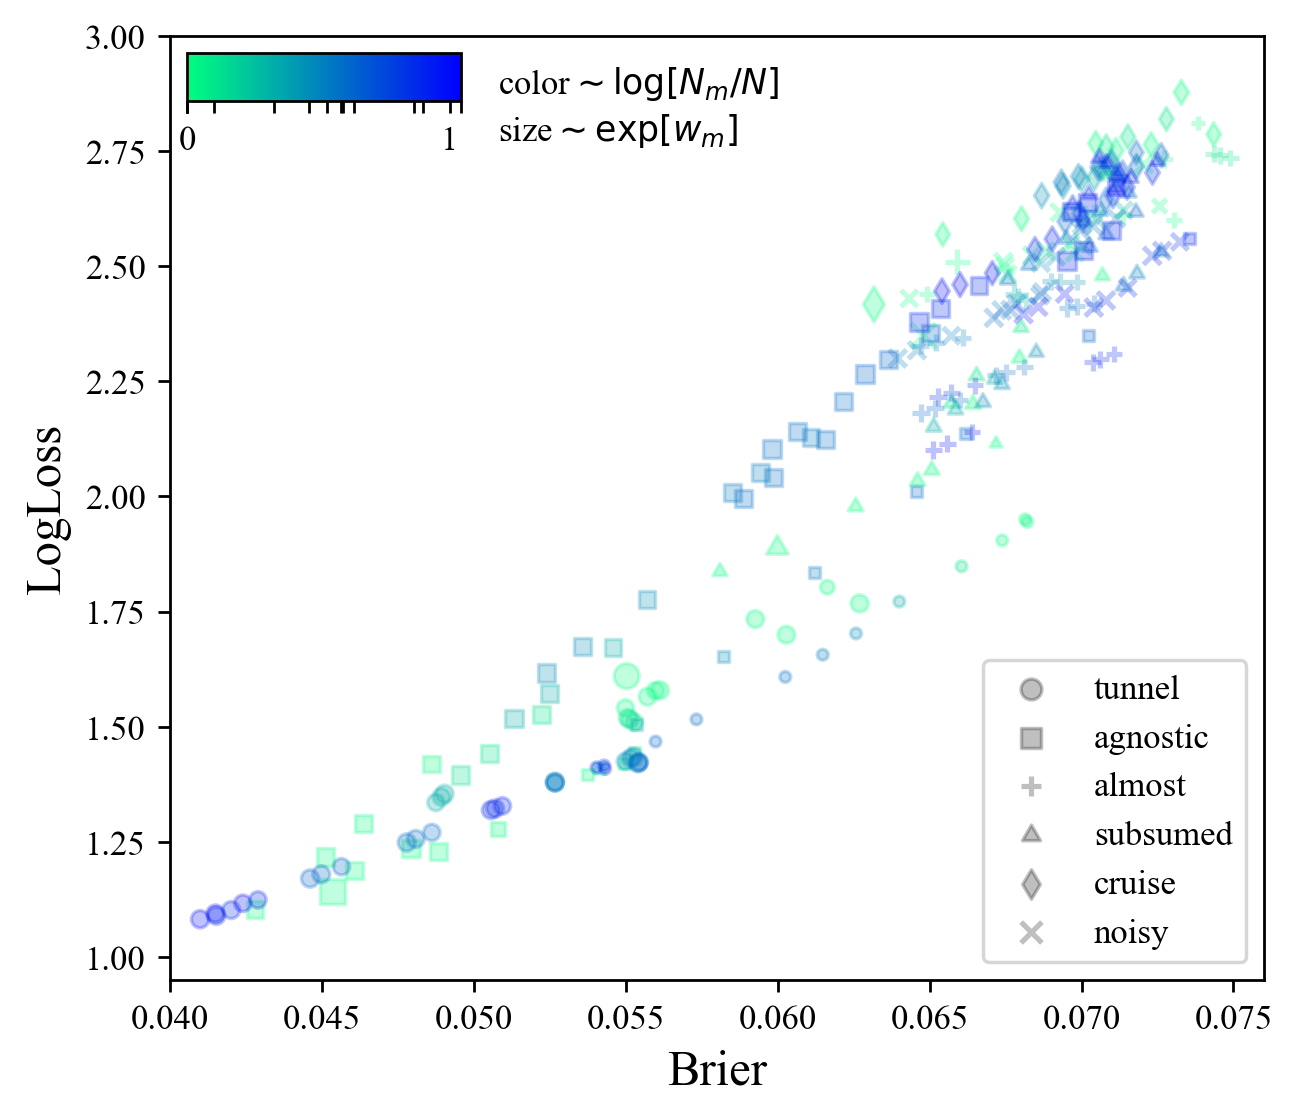
\includegraphics[width=0.5\textwidth]{./fig/all_effects_isolated.png}
% 		\caption{Population-weighted log-loss and Brier scores for classifiers with one class affected by a systematic, as a function of the population of the affected class.
% 		Each point corresponds to an almost perfect classifier that with one class instead affected by a systematic (shape), with log-loss on the $y$ axis and Brier score on the $x$ axis.
% 		The metrics are calculated with a weighting (color and size) proportional to the log of its weight in a weighted average following Equation~\ref{eq:weightavg}.
% 		}
% 	\end{center}
% 	\label{fig:popweight}
% \end{figure}

The tunnel vision classifier has a consistently low value under the Brier score and log-loss metric (bottom left corner of the plot), only increasing its Brier score once the weighting drops (less blue).
In this view, the Brier score appears to be more susceptible to tunnel vision than the log-loss, demonstrating a more significant decrease as the size of the affected class increases, but both metrics have concerning behavior in this regard.
This finding suggests that weighting alone may not be sufficient to counter the influence of this effect, and indicates a need for another balancing mechanism, such as requiring a threshold metric value on all classes.
% When considering a method of converting from one of these metrics to a finall `winner' of the classification challenge, care must be taken to ensure that all approaches do reasonably well at classifying more than one object.
% This thresholding procedure is discussed in the text

% \textbf{Ashish to reaplce/add more here?}
%\aim{Preliminary results indicate weighting will be very important for preventing the tunnel vision classifier from winning. It may be necessary to a priori anticipate which classes will have to be most strongly protected from this systematic via upweighting them.}

%\begin{figure}
%	\begin{center}
%		% 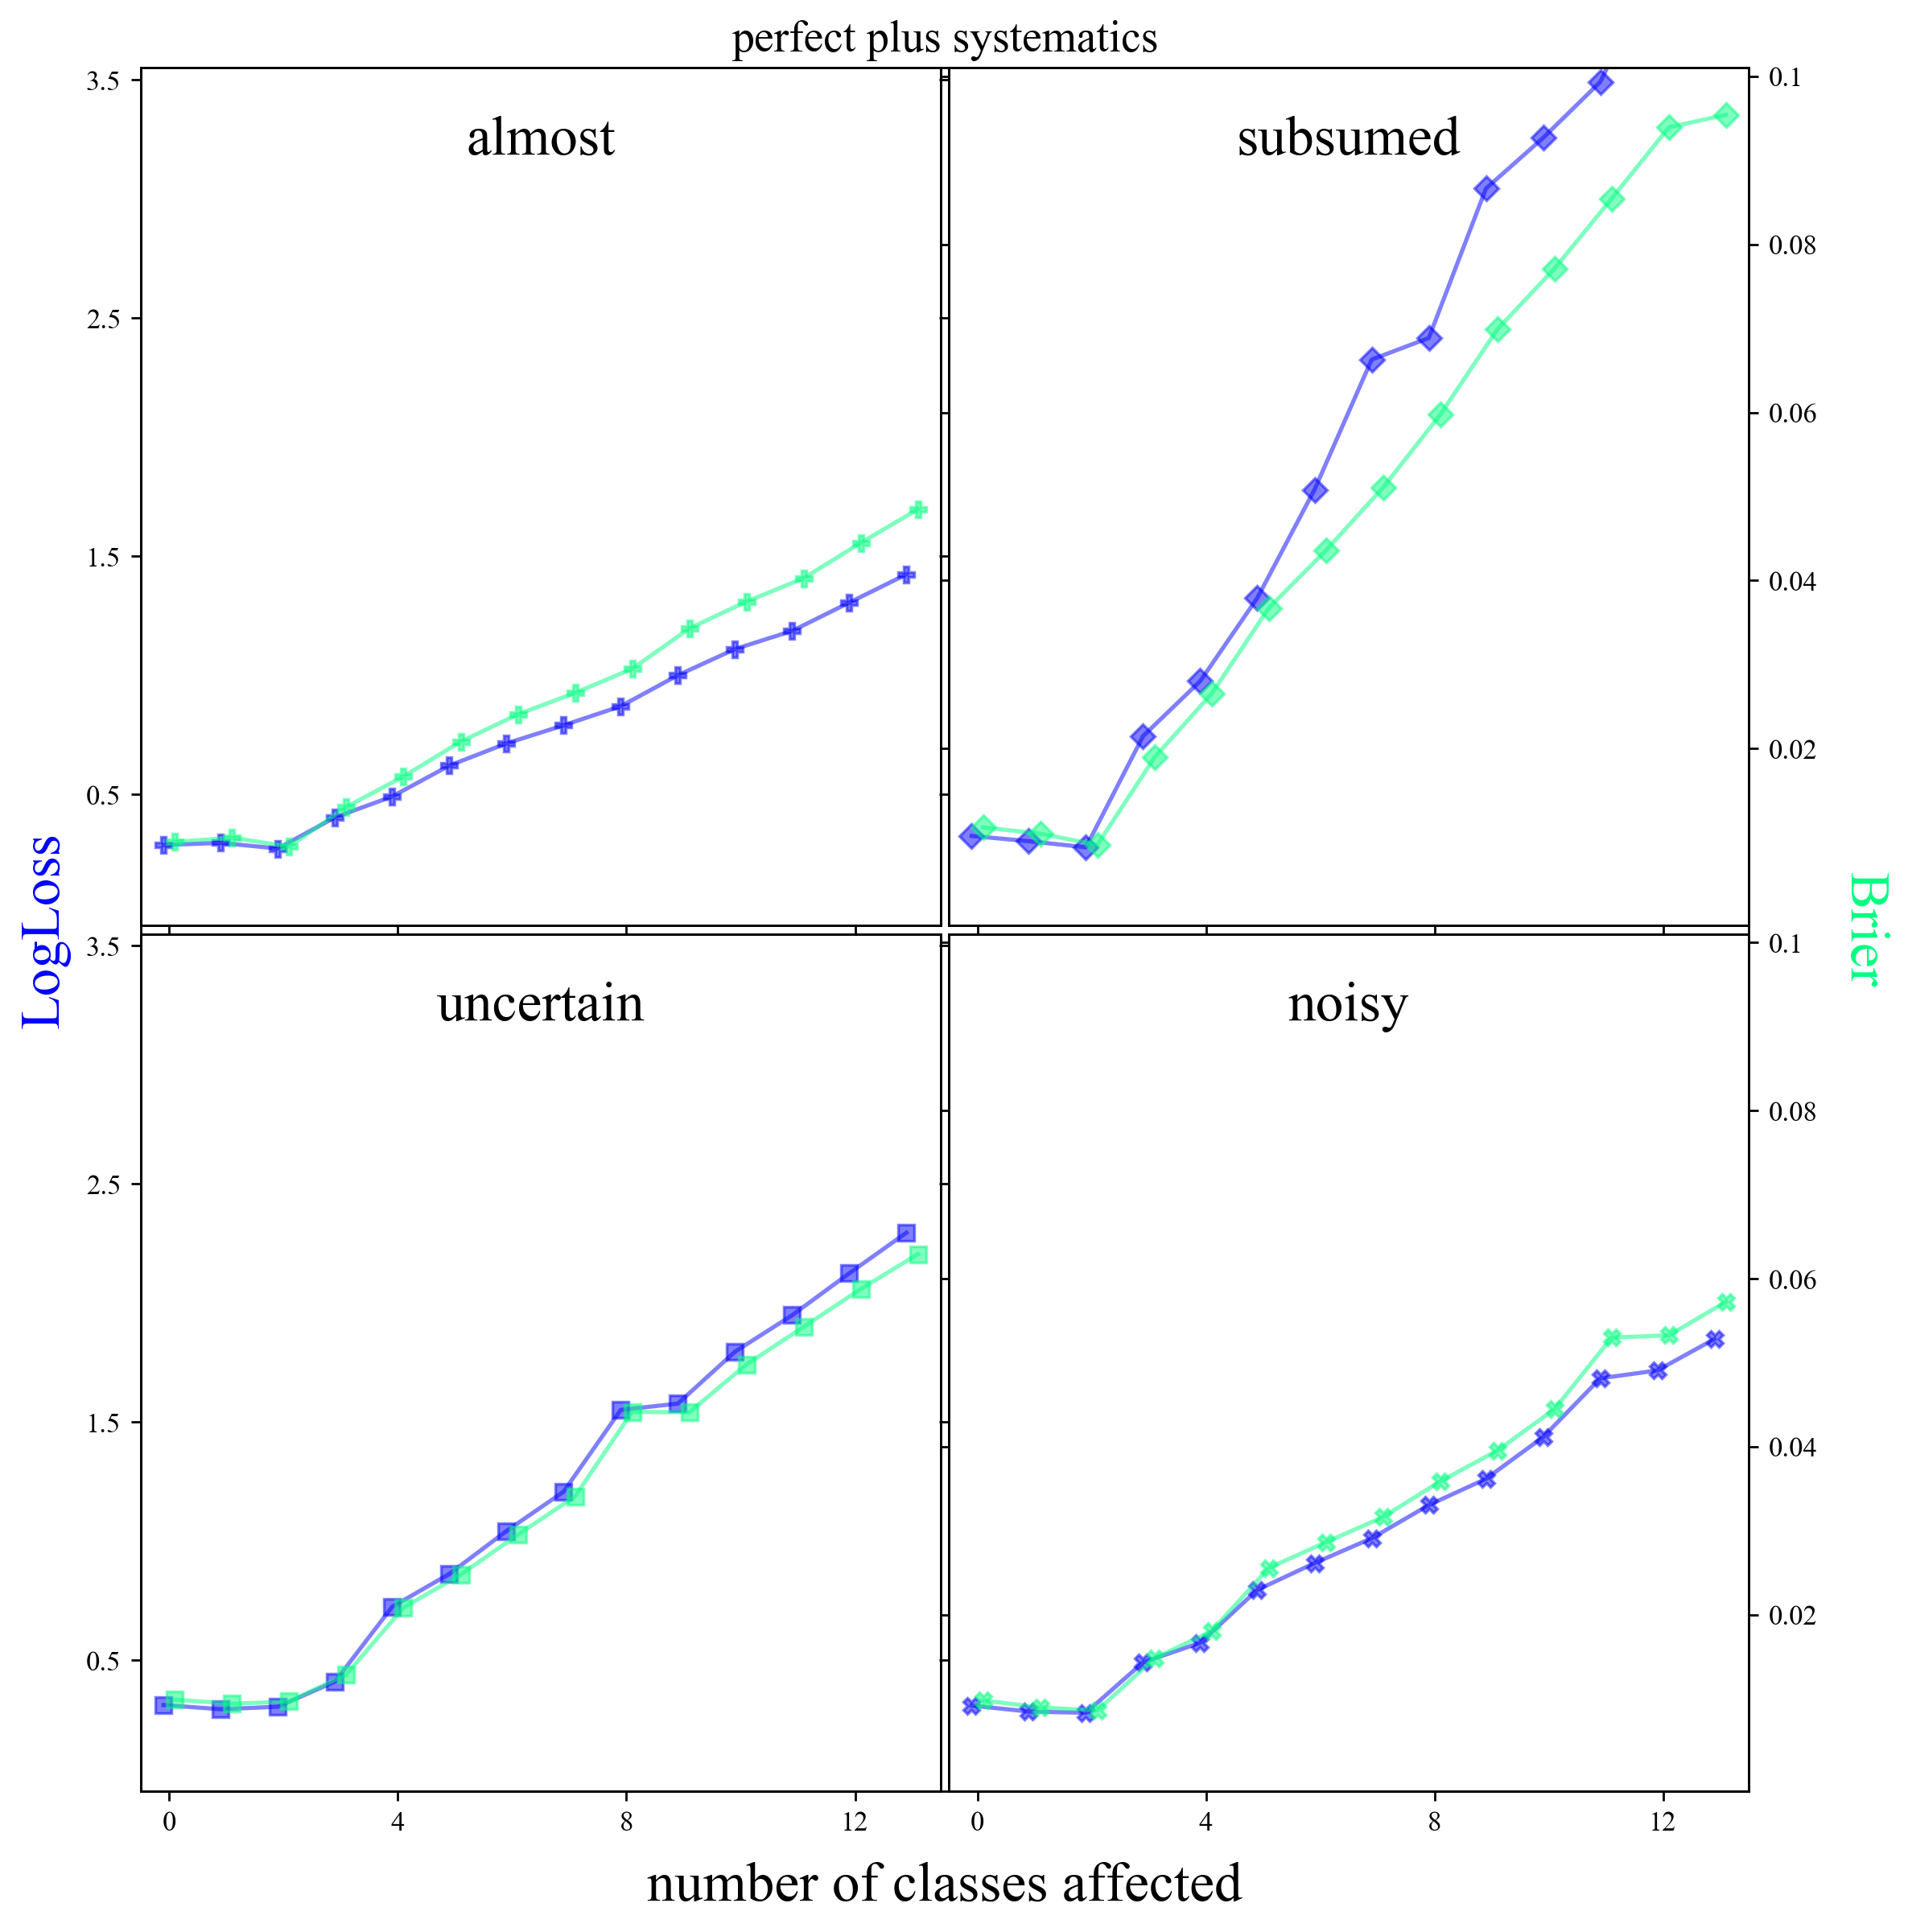
\includegraphics[width=0.5\textwidth]{./fig/systematics_onlyperfect.png}
%		\caption{\aim{After much iteration on how best to present these tests, a figure similar to Figure~\ref{fig:cruise} but for the tunnel vision classifier (heading) on different baseline classifications (panels) as a function of weight on the affected class (rather than number of classes) is under construction.}}
%		\label{fig:tunnel}
%	\end{center}
%\end{figure}

\subsection{Representative classifications}
\label{sec:realresults}

We also present in Table~\ref{tab:snmachinevals} the values of all metrics we considered, under equal weight per object, for classification probabilities derived from running the algorithms of \citet{lochner_photometric_2016} on the \snphotcc\ data of Section~\ref{sec:realdata}.
Table~\ref{tab:snmachinerank} shows the ranking of classifier performance under each metric.

\begin{table}[]
\begin{tabular}{llll}
%                            & AUC    & Brier   & FoM   & Logloss            \\
% templates\_bf  						 & 0.982 & 0.0486  & 0.635  & 0.0907  \\
% templates\_knn             & 0.942 & 0.0787  & 0.384 & 0.146  \\
% templates\_nb              & 0.879 & 0.105  & 0.340  & 0.251 \\
% templates\_nn							 & 0.954 & 0.0650  & 0.496   & 0.125 \\
% templates\_svm             & 0.969 & 0.0583 & 0.514  & 0.113 \\
% wavelets\_bf   						 & 0.978 & 0.0689  & 0.591  & 0.1321 \\
% wavelets\_knn              & 0.894 & 0.132  & 0.114 & 0.228 \\
% wavelets\_nb               & 0.850 & 0.178  & 0.0365 & 0.443  \\
% wavelets\_nn 							 & 0.946 & 0.0750  & 0.480  & 0.152 \\
% wavelets\_svm              & 0.968  & 0.0730  & 0.499  & 0.1316
& Brier   & FoM   & Logloss            \\
\hline
templates\_bf  						 & 0.0486  & 0.635  & 0.0907  \\
templates\_knn             & 0.0787  & 0.384 & 0.146  \\
templates\_nb              & 0.105  & 0.340  & 0.251 \\
templates\_nn							 & 0.0650  & 0.496   & 0.125 \\
templates\_svm             & 0.0583 & 0.514  & 0.113 \\
wavelets\_bf   						 & 0.0689  & 0.591  & 0.1321 \\
wavelets\_knn              & 0.132  & 0.114 & 0.228 \\
wavelets\_nb               & 0.178  & 0.0365 & 0.443  \\
wavelets\_nn 							 & 0.0750  & 0.480  & 0.152 \\
wavelets\_svm              & 0.0730  & 0.499  & 0.1316 \\
\end{tabular}
\caption{The values of three metrics for each of ten \snmachine\ classifiers with equal weight per object.}
	\label{tab:snmachinevals}
\end{table}

\begin{table}[]
\begin{tabular}{llll}
%   & AUC             & Brier           & FoM             & Logloss       \\
% 1 & templates\_bf 	& templates\_bf	 	& templates\_bf 	& templates\_bf \\
% 2 & wavelets\_bf	 	& templates\_svm 	& wavelets\_bf		& templates\_svm \\
% 3 & templates\_svm 	& templates\_nn 	& templates\_svm	& templates\_nn \\
% 4 & wavelets\_svm 	& wavelets\_bf 		& wavelets\_svm		& wavelets\_svm \\
% 5 & templates\_nn 	& wavelets\_svm 	& templates\_nn		& wavelets\_bf \\
% 6 & wavelets\_nn 		& wavelets\_nn 		& wavelets\_nn		& templates\_knn \\
% 7 & templates\_knn 	& templates\_knn 	& templates\_knn	& wavelets\_nn \\
% 8 & wavelets\_knn 	& templates\_nb 	& templates\_nb		& wavelets\_knn \\
% 9 & templates\_nb 	& wavelets\_knn 	& wavelets\_knn		& templates\_nb \\
% 10 & wavelets\_nb 	& wavelets\_nb 		& wavelets\_nb		& wavelets\_nb \\
Rank & Brier           & FoM             & Logloss       \\
\hline
1 & templates\_bf	 	& templates\_bf 	& templates\_bf \\
2 & templates\_svm 	& wavelets\_bf		& templates\_svm \\
3 & templates\_nn 	& templates\_svm	& templates\_nn \\
4 & wavelets\_bf 		& wavelets\_svm		& wavelets\_svm \\
5 & wavelets\_svm 	& templates\_nn		& wavelets\_bf \\
6 & wavelets\_nn 		& wavelets\_nn		& templates\_knn \\
7 & templates\_knn 	& templates\_knn	& wavelets\_nn \\
8 & templates\_nb 	& templates\_nb		& wavelets\_knn \\
9 & wavelets\_knn 	& wavelets\_knn		& templates\_nb \\
10 & wavelets\_nb 		& wavelets\_nb		& wavelets\_nb \\
\end{tabular}
\caption{The ranking of the classifiers of Table~\ref{tab:snmachinevals} under each metric.}
\label{tab:snmachinerank}
\end{table}
% TODO tell Michelle there's definitely a bug in her logloss!

The FOM of Equation~\ref{eq:snphotccfom} differs more from the Brier and log-loss metrics than they do from one another, but all three metrics are in agreement over the winners and losers, indicating that both of the potential \plasticc\ metrics are roughly consistent with our intuition about what makes a good classifier.

%\textbf{Current plan is that we compute the SNPhotCC metric for Michelle's contributions and also turn the binary classifications into probabilities - Renee will flesh this out}
%\aim{We are still iterating on the most informative tests to conduct on the \snphotcc\ data.
%I would like to have the confusion matrices from a real classification challenge (\snphotcc\ or Ashish Mahabal's) and test different weightings of our metrics on mock classification probabilities derived from those confusion matrices to check whether we choose the same ``winner,'' but the arrangements have not yet been finalized.
%The ``pipeline,'' however, is complete and ready to run as soon as the test conditions are agreed upon.}
